\documentclass[10pt,a4paper]{article}
\usepackage[margin=18mm]{geometry}
\usepackage[T1]{fontenc}
\usepackage{lmodern,microtype,graphicx,booktabs,array,amsmath,amssymb,xcolor,caption,fancyhdr,enumitem}
\usepackage[colorlinks=true,linkcolor=blue!45!black,urlcolor=blue!55!black,citecolor=blue!45!black]{hyperref}
\hypersetup{pdftitle={Online Machine Learning with River and CapyMOA},pdfauthor={Tianyi LIANG}}
\graphicspath{{figures/}}
\setlength{\parindent}{0pt}
\setlength{\parskip}{5pt}
\setlist[itemize]{nosep,leftmargin=15pt}
\captionsetup{font=small,labelfont=bf,skip=4pt,hypcap=false}
\pagestyle{fancy}\fancyhf{}\fancyhead[L]{\small Online Machine Learning with River and CapyMOA}\fancyhead[R]{\small Tianyi LIANG}\fancyfoot[C]{\thepage}
\setlength{\headheight}{14pt}
\newcommand{\resulttable}[3]{\begin{center}\captionof{table}{#2}\label{tab:#1}\vspace{2pt}{\fontsize{7.3}{9}\selectfont\setlength{\tabcolsep}{3.2pt}\input{tables/#1.tex}}\end{center}}
\newcommand{\resultfigure}[3]{\begin{center}\includegraphics[width=#3\linewidth]{#1.pdf}\captionof{figure}{#2}\label{fig:#1}\end{center}}
\begin{document}
\thispagestyle{empty}
{\LARGE\bfseries Online Machine Learning\\[3pt]with River and CapyMOA}\par
{\large A step-by-step experimental study}\par
Tianyi LIANG \hfill 13 November 2026\\
ENSTA Paris
\vspace{5pt}\hrule\vspace{5pt}
\textbf{Scope.} This report follows Steps 1--9 and optional Step 10 of the lab \cite{lab}: prediction, computational cost, drift handling, streaming clustering and online AutoML. All results come from saved experimental outputs. The repository includes code, environment configuration, summary results, figures and this \LaTeX{} source.\par
The results favor different models in different regimes. Adam regression has the lowest RMSE on three of four streams, while KNN is strongest on TrumpApproval. River KNN reaches 87.44\% accuracy on Elec2. Resetting a tree improves synthetic drift recovery, but frequent resets can degrade real-stream accuracy. CapyMOA accelerates the configured bagging ensemble; its linear learner uses a different optimizer and adapts poorly to the synthetic reversal. Online AutoML incurs substantial selection overhead and does not exceed the best static candidate in these runs.
\section{Steps 1 and 7: environment and shared evaluation}
River provides incremental Python learners; CapyMOA connects Python to MOA and other learning backends \cite{river,capymoa}. Experiments use River 0.26.1, CapyMOA 0.15.1, Python 3.11.18, OpenJDK 17.0.18 and scikit-learn 1.9.1 on an Apple M4 Pro with 48 GiB RAM. Each run executes in a separate process, sequentially, with numerical thread limits set to one and a 2 GiB Java heap limit. Installation checks cover regression, classification, drift updates and Java clustering.

\textbf{Data coverage.} All real datasets in Table~\ref{tab:data} are used in full. Chronological sources retain their order. Phishing and BreastCancer have no assumed temporal ordering, so their complete rows are permuted independently using seed 42. Identical cached streams are supplied to both libraries. Seed 42 controls data generation/permutation and stochastic learners; temporal real streams retain their source chronology.
\begin{center}\captionof{table}{Supervised data. Counts include the 50-instance training-only warm-up.}\label{tab:data}
\small\begin{tabular}{llrrl}\toprule
Task & Dataset & $N$ & Features & Stream order / target\\\midrule
Regression & TrumpApproval & 1,001 & 6 & Time / approval rating\\
& ChickWeights & 578 & 5 & Time / chick weight\\
& BikeDaily (UCI) & 731 & 34 & Date / daily rental count\\
& FriedmanShift & 10,000 & 10 & Generated / continuous response\\\midrule
Classification & Elec2 & 45,312 & 8 & Source order / price direction\\
& Phishing & 1,250 & 9 & Seeded permutation / website class\\
& BreastCancer & 569 & 30 & Seeded permutation / diagnosis\\
& SEAReversal & 10,000 & 3 & Generated / binary concept\\\bottomrule
\end{tabular}\end{center}
TrumpApproval and ChickWeights are supplied by River; BikeDaily is the 731-row daily file of the UCI Bike Sharing collection \cite{datasets,bike}. Phishing and Elec2 use River's copies. BreastCancer uses scikit-learn's 569-row Wisconsin Diagnostic dataset \cite{sklearn}. Chick identity is excluded and diet is one-hot encoded. Bike calendar/weather categories are one-hot encoded; the ID, date and target components \texttt{casual} and \texttt{registered} are excluded. The latter two would reveal the rental-count target through their sum.

\textbf{Warm-up and scaling.} The first 50 observations train each learner but are not scored. Feature means and population standard deviations are fitted only on this prefix and then held fixed. Regression targets are standardized with the same prefix; predictions are converted back to original units for evaluation. This avoids future-data leakage and keeps stored KNN observations in a fixed coordinate system.

\textbf{Evaluation.} The fixed seed is 42. For each scored example, predict before training. Regression reports MAE, RMSE and $R^2$ in original target units; classification reports accuracy, macro-F1 and Cohen's $\kappa$. Missing predictions map to class 0 or the warm-up target mean. A single fixed seed meets the lab's reproducibility requirement; these results do not estimate between-seed variation.

\textbf{Cost.} Latency includes input conversion, prediction, learning and any detector/reset operation. It excludes shared loading/scaling, package/JVM startup, warm-up, final scoring and disk output. Evaluation runtime also includes bookkeeping and memory sampling. Whole-process RSS is sampled every 250 examples and at completion; it includes Python/JVM overhead and may miss short-lived peaks. No hyperparameter search is performed.
\clearpage
\section{Steps 2--3: River regression comparison}
The four families are HoeffdingTreeRegressor (HT), Adaptive Random Forest (ARF, ten trees), LinearRegression with Adam(.01) and intercept step .01, and KNNRegressor ($k=5$, recent window 500). Trees use mean leaves, grace period 50, $\delta=10^{-7}$ and tie threshold .05. ARF retains native random subspaces, resampling and internal drift handling. HT partitions the feature space incrementally, Adam fits a linear response, and KNN adapts by forgetting old examples.
\resulttable{regression}{Full-stream prequential regression with seed 42. RSS is sampled whole-process MiB. Lower MAE/RMSE and higher $R^2$ are better.}{unused}
\resultfigure{regression-learning}{Cumulative RMSE over the complete scored stream, seed 42. The dotted vertical line marks the synthetic change at index 5000. Each panel has its own target units and vertical scale.}{.94}
\textbf{Accuracy versus cost.} LinearAdam gives the lowest RMSE on ChickWeights (39.70), BikeDaily (858.93) and FriedmanShift (2.88), at 6.2, 18.7 and 7.9 microseconds per example. On BikeDaily its RMSE is 33.4\% below ARF's 1290.44, while its evaluation runtime is 0.013 versus 0.580 seconds. This setting rewards rapid coefficient updates more than the extra capacity of a slowly growing ensemble.

TrumpApproval instead favors KNN: RMSE 0.444 versus 0.604 for LinearAdam. Its local memory captures relationships among contemporaneous approval measures; the linear model remains the faster alternative. ARF improves substantially over the single mean-leaf tree on every stream, but adds resampling and multi-tree update costs. On FriedmanShift it takes 11.73 seconds versus 0.08 seconds for LinearAdam.

The HT has negative $R^2$ on TrumpApproval and BikeDaily, meaning its squared error exceeds that of the retrospective constant target mean. Its conservative splits and mean leaves are a weak configuration for these short, evolving regression streams. Figure~\ref{fig:regression-learning} also shows why a single final score is insufficient: the synthetic reversal interrupts learning, and the methods recover at different rates.
\clearpage
\section{Step 4: regression drift detection and handling}
The synthetic response follows $f(x)=10\sin(\pi x_0x_1)+20(x_2-.5)^2+10x_3+5x_4+\epsilon$, with independent uniform $[0,1]$ features and $\epsilon\sim N(0,1)$. At index 5000 the target becomes $30-f(x)$. The feature distribution remains fixed; the conditional response changes abruptly.

ADWIN, Page--Hinkley and KSWIN monitor the same no-reset HT residual stream. Their input is $\min(|y_t-\hat y_t|/(3\sigma_{\rm warmup}),1)$. ADWIN compares adaptive-window means; Page--Hinkley accumulates deviations; KSWIN compares recent error distributions. Parameters are ADWIN $\delta=.002$; Page--Hinkley threshold 50, tolerance .005, forgetting .9999, minimum 30; KSWIN $\alpha=.005$, window 100, test sample 30. A detector restarts after an alarm. Exact positions for all streams are saved in \texttt{results/tables/detector-alarms.json}.
\resulttable{regression-drift}{Common-HT detector alarms and separate live-reset effects. First/last: zero-based alarm indices; Pre: pre-change count; Hit/Delay: post-change detection and delay in observations. $\Delta$: relative RMSE reduction versus no-reset HT. Post: reset-policy post-change RMSE. Real-stream change locations are unlabelled: Pre/Hit/Delay are not applicable (--), not zero.}{unused}
\resultfigure{regression-drift}{Top: 250-instance rolling RMSE for the no-reset HT and live reset policies (seed 42). Bottom: detector-only alarm positions on the unchanged baseline error trace. These two panels evaluate distinct detector uses.}{.94}
\textbf{Detection speed is not the same as adaptation benefit.} On FriedmanShift, KSWIN raises its first post-change alarm after 22 observations, ADWIN after 41, and Page--Hinkley after 187. KSWIN also produces five pre-change alarms, compared with one each for the other detectors. Learning transients can alter the error distribution even before the generating concept changes.

The separate live-reset experiments reduce overall HT RMSE from 4.97 to 3.92 (ADWIN), 3.93 (Page--Hinkley) and 4.02 (KSWIN). ADWIN gives the best overall and post-change RMSE despite KSWIN's shorter baseline detection delay. KSWIN approximately doubles latency here (305 versus 155 microseconds for no reset), reflecting its distribution tests.

KSWIN resets reduce RMSE by 51.03\% on TrumpApproval and 32.49\% on BikeDaily; Page--Hinkley never alarms on either. ChickWeights triggers no detector and no reset benefit. Real-stream alarms concern prediction errors; without labelled changes, detection precision and delay cannot be measured.
\clearpage
\section{Step 5a: River classification comparison}
Classification compares HT, ADWIN bagging (ten HT members), logistic regression with Adam(.01), and unweighted KNN ($k=5$, window 500). Trees use majority leaves, information gain, grace 50, $\delta=10^{-7}$, tie threshold .05 and no pre-pruning. Logistic regression uses intercept step .01 and no L2 penalty. The same three real streams and one synthetic stream are used for all four methods. SEAReversal samples $x\sim U([0,10]^3)$, initially assigns $y=\mathbb{1}[x_0+x_1>8]$, reverses this label at index 5000, and independently flips 5\% of labels. This deliberately controlled SEA-based drift provides a known change location while leaving $P(X)$ unchanged.
\resulttable{classification}{River classification with seed 42. Accuracy and macro-F1 are percentages; $\kappa$ is dimensionless. Latency is the mean per example; runtime is total evaluation time. All methods observe every record after the shared training-only prefix.}{unused}
\resultfigure{classification-learning}{Cumulative classification accuracy, seed 42. The reversal is marked at index 5000. Static datasets use a fixed row permutation.}{.94}
\textbf{A fast linear model is often competitive, but locality matters.} KNN gives the highest Elec2 accuracy (87.44\%) and $\kappa$ (0.742). Its 500-example window can forget old conditions without explicit detector resets. Logistic regression is much faster (7.5 versus 97.5 microseconds), but its 70.23\% Elec2 accuracy shows the cost of the configured linear representation and optimization.

On Phishing, Logistic reaches 89.00\% accuracy, slightly above KNN's 88.50\%, at about one tenth of KNN's latency. On BreastCancer the pair is nearly tied (95.76\% and 95.95\%). Both tree configurations predict the majority label for all 519 scored BreastCancer observations, giving 62.24\% accuracy and zero $\kappa$. Thus this conservative majority-leaf setup is unsuitable for the short stream, rather than evidence that all tree configurations fail on the task.

On SEAReversal, Logistic and KNN achieve 89.70\% and 89.35\%, compared with 66.96\% for HT and 63.43\% for bagging. The finite KNN window and persistent Adam updates support recovery; increasing ensemble size alone does not guarantee effective adaptation under these settings.
\clearpage
\section{Step 5b: classification drift and recovery}
ADWIN, DDM and EDDM receive binary prequential errors from the same no-reset HT for the detector-only comparison. DDM tracks error probability and its variability (warm-up 30 errors, warning multiplier 2, drift multiplier 3). EDDM tracks spacing between errors (warm-up 30, warning ratio .95, drift ratio .90). Parameters are not tuned to the known synthetic drift.

For the handling ablation, each detector instead observes the errors of its own live HT. An alarm resets both learner and detector, then the current labeled example trains the new tree exactly once. The fixed scaler is retained. This separates \emph{detecting a change} from \emph{improving prediction after acting on it}.
\resulttable{classification-drift}{Alarm statistics (including first/last positions) and classification reset effects. $\Delta$ is accuracy improvement in percentage points over the no-reset HT. Post metric is post-reversal accuracy in percent. For real streams, Pre/Hit/Delay are not applicable (--): true change locations are unlabelled. A missing synthetic detection is distinct from zero delay.}{unused}
\resultfigure{classification-drift}{Top: rolling accuracy for no reset and three live reset strategies on SEAReversal. Bottom: alarms obtained from the common no-reset error trace. Results shown for seed 42; the table reports the same run.}{.94}
\textbf{The reset rule changes the outcome.} On the common SEAReversal baseline errors, ADWIN detects the change after 41 observations, DDM after 96 and EDDM after 253. EDDM has already raised 11 pre-change alarms. Faster detection does not translate monotonically into better accuracy once the detector is coupled to a changing learner.

DDM resets raise overall accuracy from 66.96\% to 77.55\% and post-change accuracy from 60.20\% to 71.54\%. ADWIN improves the post-change portion to 66.26\%, but its overall accuracy falls slightly to 66.70\%; gains after the reversal do not offset losses elsewhere. EDDM ends at 66.04\% overall.

On Elec2 all three live-reset policies are worse than retaining the HT, by 8.78, 3.18 and 6.32 percentage points for ADWIN, DDM and EDDM. Restarting repeatedly discards learned structure and imposes relearning costs. Phishing shows a different outcome: EDDM gains 8.33 points while ADWIN loses 8.83. These comparisons support evaluating a complete detector--learner policy, rather than selecting a detector solely by its alarm count or synthetic detection delay.
\clearpage
\section{Step 8: River versus CapyMOA}
Both libraries receive the same arrays, feature scaling, warm-up and observation order. CapyMOA uses HoeffdingTree, OnlineAdwinBagging, SGDClassifier with logistic loss, and KNN, matching the explicit tree settings, ensemble size, $k$ and window. Its logistic wrapper uses inverse-scaling SGD ($\eta_t=.01/t^{.5}$), not Adam \cite{sgd}. This is a closest-equivalent linear-family comparison; native split observers, distance normalization, random-number generators and internal drift logic can also differ. Table~\ref{tab:cross-library} pairs results by dataset and model family. R/C is River latency divided by CapyMOA latency; values above one favor CapyMOA on this machine. The accuracy difference is CapyMOA minus River. The paired linear implementations intentionally retain their native optimizers as documented in the model descriptions.
\resulttable{cross-library}{Cross-library accuracy, total evaluation time (seconds) and mean latency (microseconds per example). R/C is the latency ratio. Native implementation differences remain part of the comparison.}{unused}
\resultfigure{cross-library}{Accuracy--cost trade-offs. Colors identify learner families; circles denote River and triangles CapyMOA. Horizontal axes are logarithmic. Each point is one complete seed-42 run.}{.94}
\textbf{Performance depends on the model family.} CapyMOA bagging is faster on all four streams: its latency advantage ranges from 2.04$\times$ to 4.19$\times$. It also improves accuracy by 4.34 points on Elec2 and 10.54 on SEAReversal, while matching the majority-class result on BreastCancer. This favors its configured ensemble implementation, not a blanket claim that every CapyMOA learner is faster.

HT accuracy matches exactly on three streams, but latency favors River on Phishing and SEAReversal. River KNN is more accurate on Elec2 (87.44\% versus 84.29\%), whereas CapyMOA KNN is faster there (61.3 versus 97.5 microseconds). Different native distance handling and tree/ensemble internals remain part of these comparisons.

The largest discrepancy is linear adaptation: CapyMOA Logistic reaches 85.31\% on Elec2, but only 48.89\% on SEAReversal. Its post-reversal accuracy is 9.36\%, versus 87.06\% for River Adam. The shrinking inverse-scaling step is consistent with poor adaptation after a late reversal; this optimizer mismatch prevents interpreting the gap as intrinsic library quality. Median sampled RSS across classification configurations is about 319 MiB for CapyMOA and 161 MiB for River, including runtime overhead.
\clearpage
\section{Step 9: streaming clustering}
Three CapyMOA methods process full Iris (150 rows, labels hidden) and MovingBlobs (6000 two-dimensional points). MovingBlobs contains three equally sampled Gaussian groups with noise SD .55; their centers translate by $(3,1.5)$ at index 3000. CluStream compresses observations into 30 microclusters and extracts $k=3$ macroclusters by $k$-means. ClusTree incrementally indexes microclusters in a tree (horizon 1000, height 3). DenStream groups fading density microclusters, using $\epsilon=.6$, $\beta=.2$, $\mu=2$, initialization 50, offline multiplier 2, decay .01 and speed 100; all methods use horizon 1000 where applicable.

After a 50-point warm-up, \emph{block-prequential} evaluation freezes current centers, assigns the next 25 Iris or 250 MovingBlobs points, evaluates them, and only then trains on that block. Labels are used solely for ARI, never learner updates. Metrics are silhouette, adjusted Rand index (ARI), and squared nearest-center distance; undefined values remain missing. ClusTree exposes microcenters, unlike the other macrocluster partitions. Nearest-center assignment evaluates DenStream's centers, not its native noise rejection. A constant Java class placeholder is used for transport only.
\resulttable{clustering}{Weighted block-quality means, for seed 42. Lower squared distance is better; higher silhouette and ARI are better. Clustering latency includes center extraction and quality computation, unlike supervised latency.}{unused}
\resultfigure{cluster-evolution}{Quality and partition size over MovingBlobs (seed 42). The dotted line marks the center translation; the block beginning 2800 spans that change.}{.95}
\resultfigure{cluster-snapshots}{CluStream centers (black crosses) before training each displayed block, overlaid on the next held-out points. Point colors/shapes indicate reference groups solely for visualization. Coordinates use the fixed warm-up scaler.}{.95}
\textbf{Cluster resolution changes metric interpretation.} CluStream has the best ARI on Iris (0.641) and MovingBlobs (0.890). On MovingBlobs its squared distance rises to 1.470 in the block starting at 3050, then falls to 0.092 in the final block as centers recover. The snapshots show the displacement directly.

ClusTree's many microcenters minimize distance (0.055 on MovingBlobs), but fragment the reference groups, lowering ARI to 0.428. DenStream has higher Iris silhouette than CluStream (0.590 versus 0.445), yet lower ARI (0.455 versus 0.641): compact separation need not recover the reference labels. Under the fixed radius/decay settings it eventually merges MovingBlobs into one macrocluster. Its first MovingBlobs block has no centers; distance/ARI use 23 of 24 blocks, and silhouette uses only 12 of 24 blocks with at least two occupied groups.
\clearpage
\section{Step 10 (bonus): online AutoML comparison}
CapyMOA's BanditClassifier uses an $\epsilon$-greedy allocation policy ($\epsilon=.1$, burn-in 100). SuccessiveHalvingClassifier starts with the same candidate pool, ranks candidates and progressively eliminates them ($\eta=2$, budget 12000 model updates, minimum one model) \cite{automl}. The pool consists of the four configured CapyMOA classifiers from Step 8. Both selectors see every stream observation, although they allocate training updates differently across candidates. The comparison covers two AutoML approaches supplied by CapyMOA; it does not evaluate AutoClass.
\resulttable{automl}{AutoML and the highest-accuracy static candidate for each dataset. The static reference is selected retrospectively from Step 8 and is not an online selection algorithm. All values use seed 42.}{unused}
\resultfigure{automl}{Left: response to the SEA label reversal for two static references and two AutoML selectors (seed 42). Right: AutoML latency across the four streams; the vertical cost axis is logarithmic.}{.95}
\textbf{Selection overhead is visible.} On Elec2, Bandit reaches 84.91\% accuracy and Successive Halving 84.26\%, close to the best static CapyMOA candidate (Logistic, 85.31\%). Their runtimes are 213.98 and 140.65 seconds, versus 21.04 seconds for that static candidate. The selectors perform additional candidate predictions, metric updates and allocation decisions; fewer active learners do not imply lower end-to-end cost in this implementation.

On SEAReversal, Successive Halving retains KNN and matches its 89.28\% accuracy, but takes 40.21 seconds versus 0.62 seconds. Bandit finishes at 48.98\% and favors the poorly adapting SGD candidate. Its cumulative reward history can preserve an earlier preference after the concept changes. Selection with a nonstationary reward mechanism would be a separate experiment.

Neither selector exceeds the retrospectively best static candidate on these four streams. That reference benefits from knowing the final result, whereas an online selector must allocate resources without this knowledge. AutoML is therefore useful here as a mechanism comparison, not an automatic accuracy or efficiency improvement. The 12000-update setting governs successive-halving elimination; the surviving candidate continues training after the selection rounds finish.
\clearpage
\section{Step 6: synthesis, reproducibility and conclusions}
\textbf{Choices supported by this experiment.} LinearAdam wins three of four regression comparisons at the lowest latency; KNN is preferable for the recent local relationships in TrumpApproval and Elec2. ARF improves over a single mean-leaf tree but costs more without achieving the best regression score here. CapyMOA is attractive for the tested ten-tree bagging ensemble, while River supplies an efficient adaptive linear learner.

For drift, evaluate the complete intervention: ADWIN resets best reduce FriedmanShift RMSE, DDM resets best improve SEAReversal accuracy, and all three reset policies harm Elec2. CluStream best recovers the reference clusters, while ClusTree's many microcenters favor coverage rather than matching three groups. The AutoML selectors add overhead without beating the retrospectively best static candidate.

\textbf{Scope.} These are seed-42 results under fixed hyperparameters, not estimates of between-seed variability. Static row permutations do not establish natural temporal drift. Optimizer differences limit cross-library attribution, desktop timings include runtime effects, and whole-process RSS is not model-only memory. Cluster reference labels describe one partition rather than a universal unsupervised ground truth.
\subsection{Reproducing the submission}
The \href{https://github.com/TimmyLTY/online-ml-river-capymoa-lab}{GitHub repository} contains the experiment code, environment, configuration, dataset manifests, summary results, exact detector positions and this self-contained report source. Reproduce on macOS from the root:
\begin{verbatim}
conda env create -f environment.yml
conda activate online-ml-lab
python src/data.py
python src/run_experiments.py
python scripts/analyze_results.py
python scripts/verify_results.py
bash scripts/build_report.sh
\end{verbatim}
The completed matrix has 86 runs: 16 regression, 32 classification, 24 resets, 6 clustering and 8 AutoML, plus 24 detector-only replays. Validation recomputes predictive metrics, checks fingerprints, and confirms paired labels and stream order. Rerunning regenerates per-instance prediction and latency traces locally; the repository retains summary evidence. The report ZIP uploads directly to Overleaf with \texttt{main.tex} and pdfLaTeX.
\par\vspace{5pt}
\noindent\begin{minipage}[t]{.44\linewidth}\vspace{0pt}
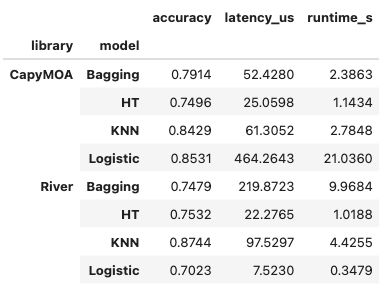
\includegraphics[width=\linewidth]{results-notebook.jpg}
\captionof{figure}{Actual executed-notebook screenshot: Elec2 results on 45,262 scored observations. Accuracy is a fraction; latency is in microseconds and runtime in seconds.}
\end{minipage}\hfill
\begin{minipage}[t]{.52\linewidth}\vspace{0pt}
\begin{thebibliography}{9}\fontsize{8.5}{10}\selectfont\setlength{\itemsep}{0pt}
\bibitem{lab} M. Barry and M. Togbe. \emph{Lab: Online Machine Learning with River and CapyMOA}. Course handout, 9 Nov. 2026.
\bibitem{river} J. Montiel et al. \emph{River: machine learning for streaming data in Python}. arXiv:2012.04740, 2020. \href{https://arxiv.org/abs/2012.04740}{Paper}.
\bibitem{capymoa} H. M. Gomes et al. \emph{CapyMOA: Efficient Machine Learning for Data Streams and Online Continual Learning in Python}. arXiv:2502.07432, 2025/2026. \href{https://arxiv.org/abs/2502.07432}{Paper}.
\bibitem{datasets} River developers. Dataset implementations and API documentation. \href{https://riverml.xyz/latest/api/datasets/Elec2/}{Dataset API}; pinned River 0.26.1 source.
\bibitem{bike} H. Fanaee-T. \emph{Bike Sharing}. UCI Machine Learning Repository. \href{https://archive.ics.uci.edu/dataset/275/bike+sharing+dataset}{Dataset record}.
\bibitem{sklearn} Scikit-learn developers. Wisconsin Diagnostic Breast Cancer and Iris dataset documentation. \href{https://scikit-learn.org/stable/datasets/toy_dataset.html}{Dataset guide}.
\bibitem{sgd} CapyMOA developers. \emph{SGDClassifier} API and implementation. \href{https://capymoa.org/api/modules/capymoa.classifier.SGDClassifier.html}{API documentation}.
\bibitem{automl} CapyMOA developers. \emph{Automated machine learning} tutorial. \href{https://capymoa.org/v0.15.0/notebooks/automl/automl.html}{Versioned tutorial}.
\end{thebibliography}
\end{minipage}
\end{document}
